% THIS DOCUMENT IS FOLLOWS THE VOLERE TEMPLATE BY Suzanne Robertson and James Robertson
% ONLY THE SECTION HEADINGS ARE PROVIDED
%
% Initial draft from https://github.com/Dieblich/volere
%
% Risks are removed because they are covered by the Hazard Analysis
\documentclass[12pt]{article}

\usepackage{booktabs}
\usepackage{tabularx}
\usepackage{hyperref}
\usepackage{graphicx}

\hypersetup{
    bookmarks=true,         % show bookmarks bar?
      colorlinks=true,      % false: boxed links; true: colored links
    linkcolor=red,          % color of internal links (change box color with linkbordercolor)
    citecolor=green,        % color of links to bibliography
    filecolor=magenta,      % color of file links
    urlcolor=cyan           % color of external links
}

\newcommand{\lips}{\textit{Insert your content here.}}

%% Comments

\usepackage{color}

\newif\ifcomments\commentstrue %displays comments
%\newif\ifcomments\commentsfalse %so that comments do not display

\ifcomments
\newcommand{\authornote}[3]{\textcolor{#1}{[#3 ---#2]}}
\newcommand{\todo}[1]{\textcolor{red}{[TODO: #1]}}
\else
\newcommand{\authornote}[3]{}
\newcommand{\todo}[1]{}
\fi

\newcommand{\wss}[1]{\authornote{blue}{SS}{#1}} 
\newcommand{\plt}[1]{\authornote{magenta}{TPLT}{#1}} %For explanation of the template
\newcommand{\an}[1]{\authornote{cyan}{Author}{#1}}

%% Common Parts

\newcommand{\progname}{Software Engineering} % PUT YOUR PROGRAM NAME HERE
\newcommand{\authname}{Team 8 -- Rhythm Rangers\\
\\ Ansel Chen
\\ Muhammad Jawad
\\ Mohamad-Hassan Bahsoun
\\ Matthew Baleanu
\\ Ahmed Al-Hayali} % AUTHOR NAMES                  

\usepackage{hyperref}
    \hypersetup{colorlinks=true, linkcolor=blue, citecolor=blue, filecolor=blue,
                urlcolor=blue, unicode=false}
    \urlstyle{same}
                                


\begin{document}

\title{Software Requirements Specification for \progname: subtitle describing software} 
\author{\authname}
\date{\today}
	
\maketitle

~\newpage

\pagenumbering{roman}

\tableofcontents

~\newpage

\section*{Revision History}

\begin{tabularx}{\textwidth}{p{3cm}p{2cm}X}
\toprule {\textbf{Date}} & {\textbf{Version}} & {\textbf{Notes}}\\
\midrule
Date 1 & 1.0 & Notes\\
Date 2 & 1.1 & Notes\\
\bottomrule
\end{tabularx}

~\\

~\newpage
\section{Purpose of the Project}
\subsection{User Business}
\lips
\subsection{Goals of the Project}
\lips
\section{Stakeholders}
\subsection{Client}
\lips
\subsection{Customer}
\lips
\subsection{Other Stakeholders}
\lips
\subsection{Hands-On Users of the Project}
\lips
\subsection{Personas}
\lips
\subsection{Priorities Assigned to Users}
\lips
\subsection{User Participation}
\lips
\subsection{Maintenance Users and Service Technicians}
\lips

\section{Mandated Constraints}
\subsection{Solution Constraints}
\lips
\subsection{Implementation Environment of the Current System}
\lips
\subsection{Partner or Collaborative Applications}
\lips
\subsection{Off-the-Shelf Software}
\lips
\subsection{Anticipated Workplace Environment}
\lips
\subsection{Schedule Constraints}
\lips
\subsection{Budget Constraints}
\lips
\subsection{Enterprise Constraints}
\lips

\section{Naming Conventions and Terminology}
\subsection{Glossary of All Terms, Including Acronyms, Used by Stakeholders
involved in the Project}
\lips

\section{Relevant Facts And Assumptions}
\subsection{Relevant Facts}
\lips
\subsection{Business Rules}
\lips
\subsection{Assumptions}
\lips

\section{The Scope of the Work}
\subsection{The Current Situation}
\begin{itemize}
  \item \textbf{Music Analysis Component}
  \\\textbf{Manual Process}: Currently, this is usually manually done by the artist self-labelling their work
  or third parties labelling the music. This can end up being time consuming. 
  \\\textbf{Automated Process}: Most automation on this regard (retrieving song information from a music 
  provider's api) is mostly useful for retreiving already labelled information, there is not a lot of automation 
  that is be done for labelling, but a lot that is possible retreiving said labels. 
  \\What we wish to do with this component of the service is to gather and present said information that can be
  gleamed from the music service provider's API to the user in a more presentable manner (such as audio visualizations)
   but also featurize an individual song for the other components in our service. Our service should also generate new
   labels using ML algorithms, which allows for faster automation of song labelling and more features for our other 
   components. 
  \\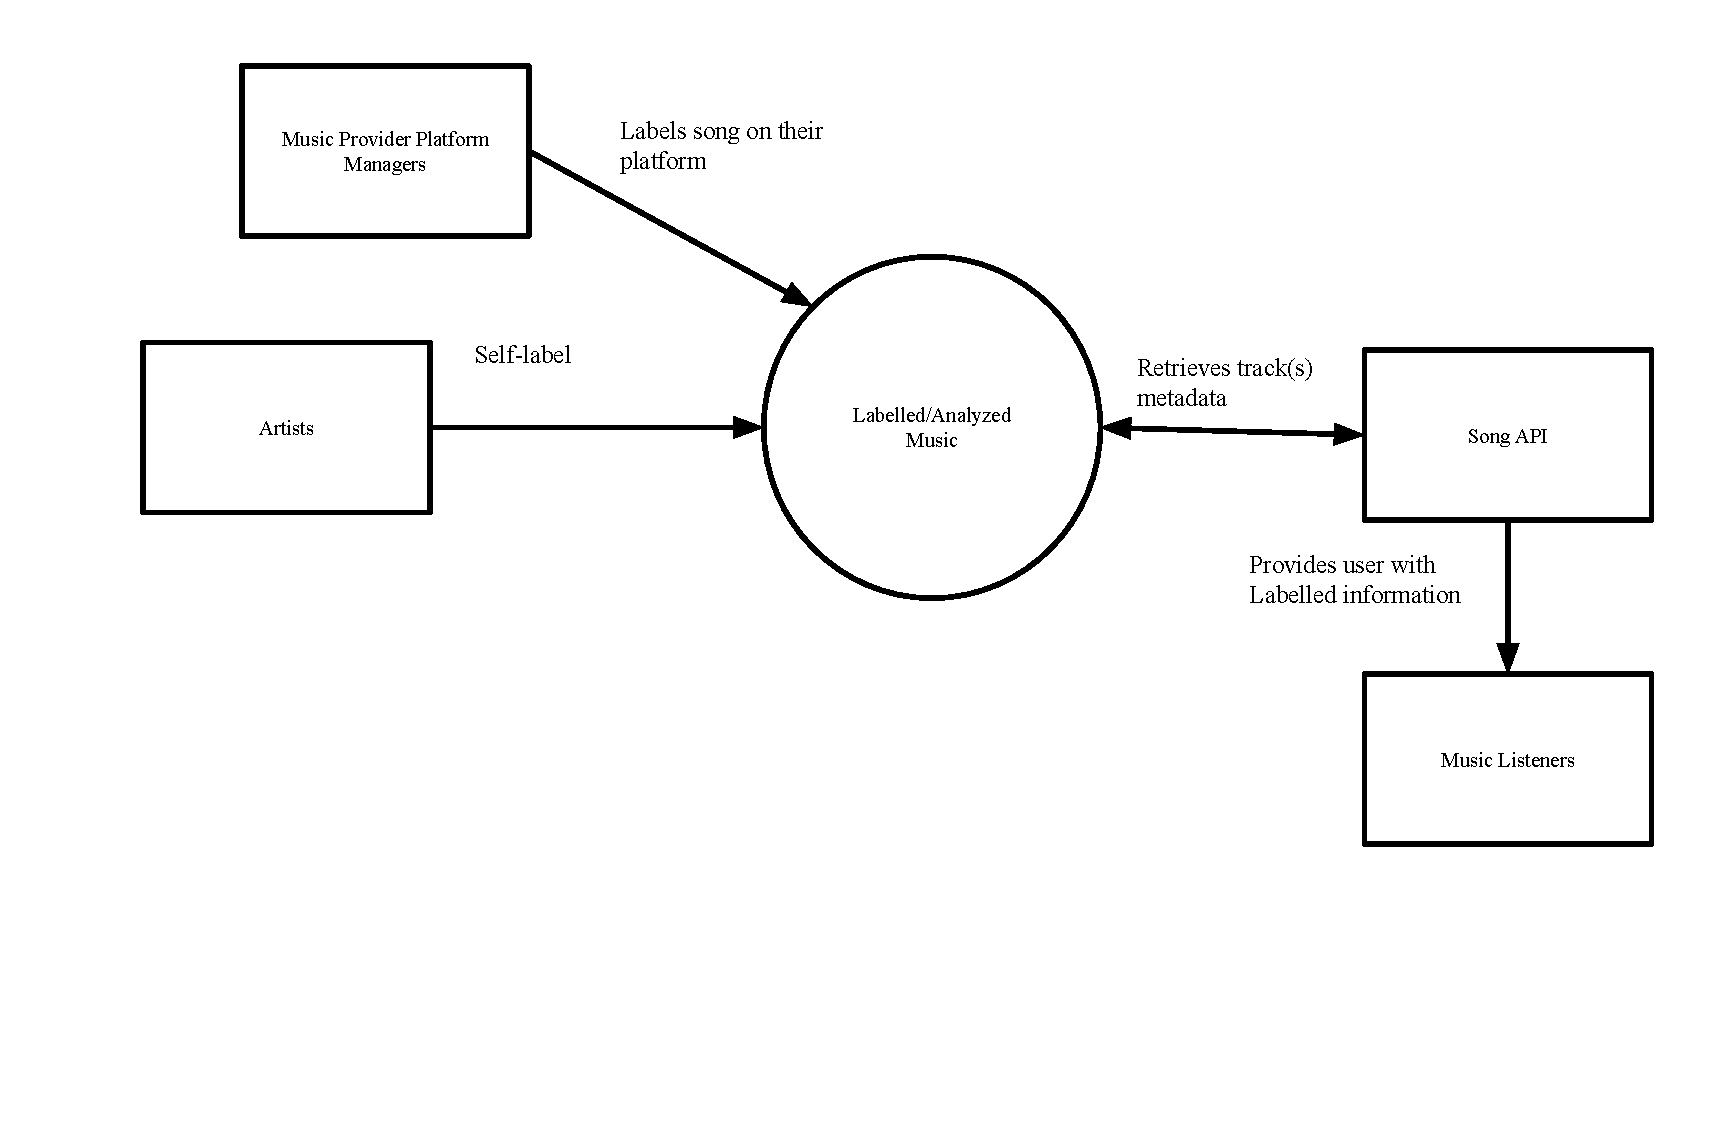
\includegraphics[width=\textwidth]{6_1_b.pdf}
  \item \textbf{Music Recommendation Component}
  \\\textbf{Manual Process}: Generally, this is mostly done through music curators should as DJs, playlist makers,
  etc, where curators manually select songs and make recommendations based on popular trends, new artists releases,
  or shifts in the genre. The main issue here is that it requires a large amount of manual work, as curators need to 
  listen to new music before adding them to some form of playlist or recommending them to other people, which greatly
  limits their potential recommendations. 
  \\\textbf{Automated Process}: Most music service providers such as spotify, apple music or youtube already offer 
  some form of music recommendation service use algorithms to recommend users new songs based on their listening history.
  These generally already work decently well, but they end up usually being heavily weighted towards more popular songs 
  (for example, sabrina carpenter's espresso being automatically recommended through smart shuffle no matter what your prior listening history was like), 
  as record labels often have deals with these music service platforms so it is not unusual to get recommendations that 
  do not necessarily suit the user's music tastes. 
  \\The main benefit our service should provide is the ability to recommend songs that are more niche, more accurate based
  on the user input while still using an automated system powered by machine learning, as we would have more features due 
  to the analysis component for the ML algorithm to process, in addition to not being heavily weighted towards more popular,
  trendy songs or some form of likely record label deals meddling. 
  \\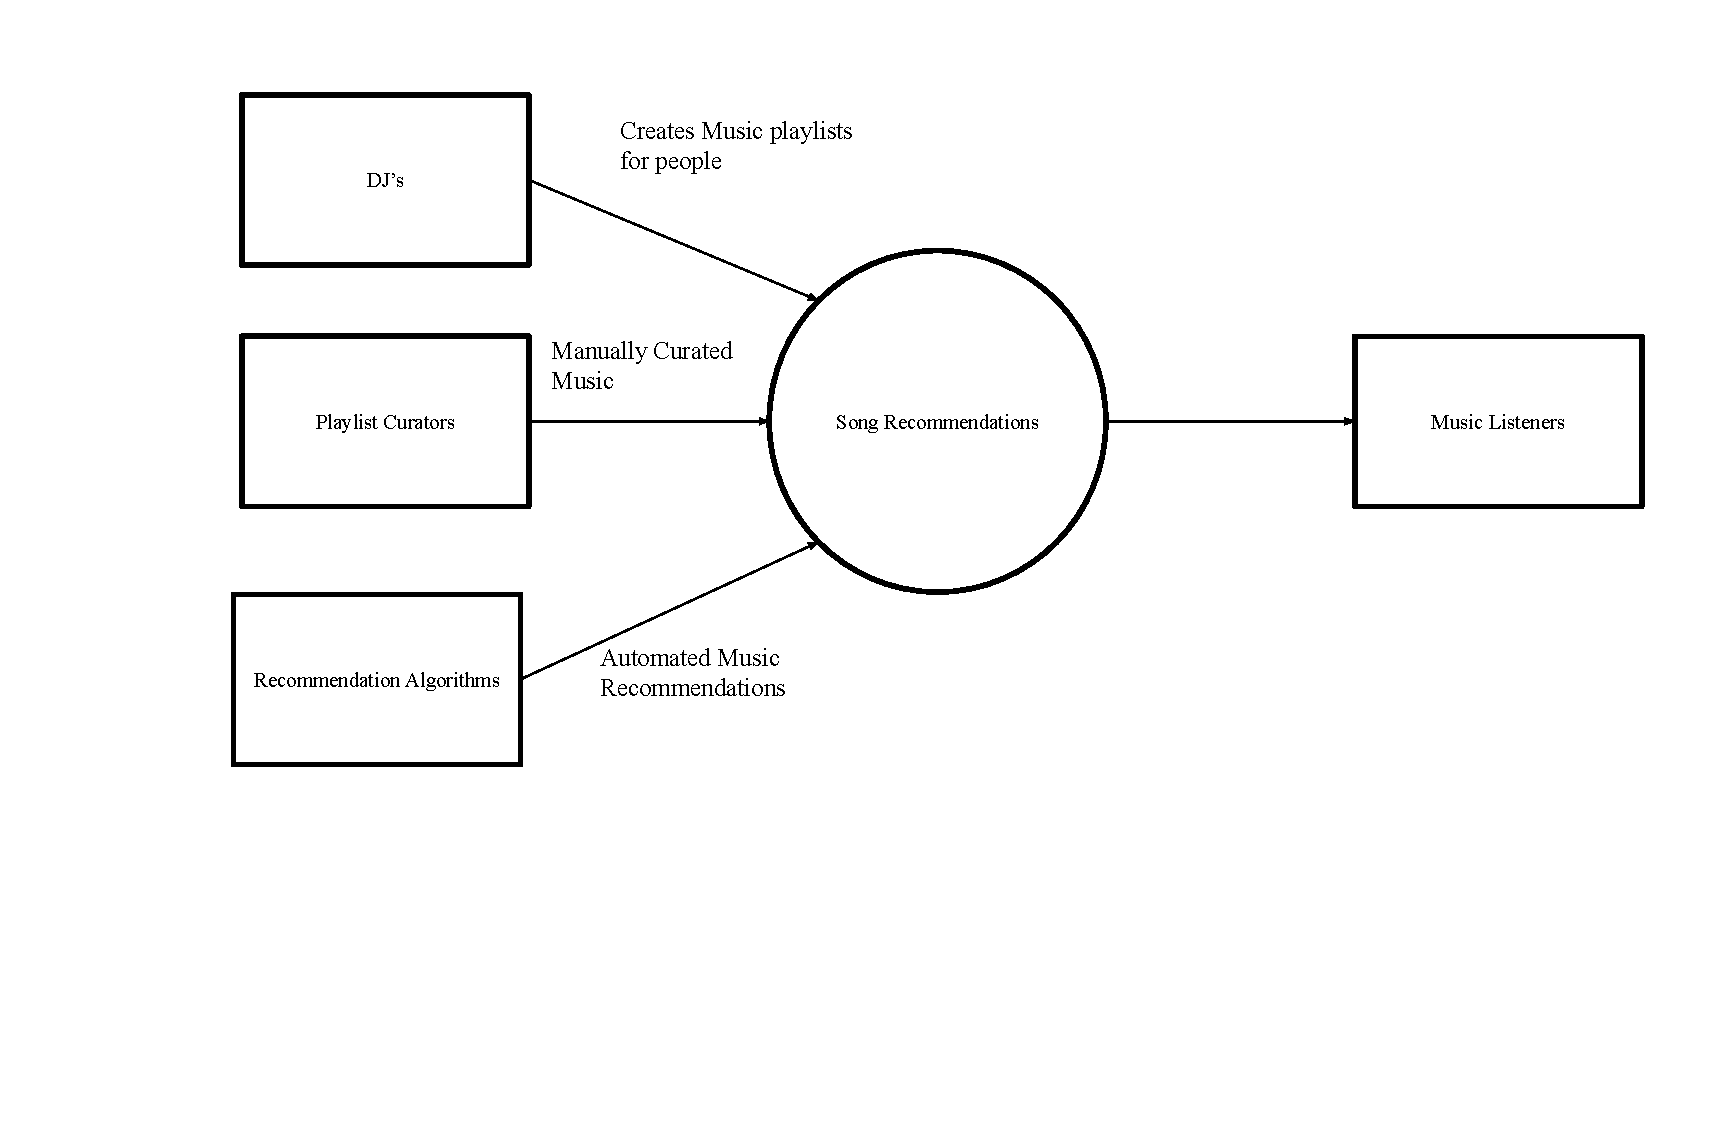
\includegraphics[width=\textwidth]{6_1_a.pdf}

  \item \textbf{Music Generation Component}
  \\\textbf{Manual Process}: Currently, generating music usually requires years of dedication to the craft and involves the
  labour of musicians, producers, and composers. This means that there is a large amount of manpower that is necessary
  in order to create new unique pieces. 
  
  We wish to have our service provide a new avenue to generate new types of music. We do not envision this service as 
  something that replaces the traditional music creation process, but rather as something that can potentially enhance it. 

  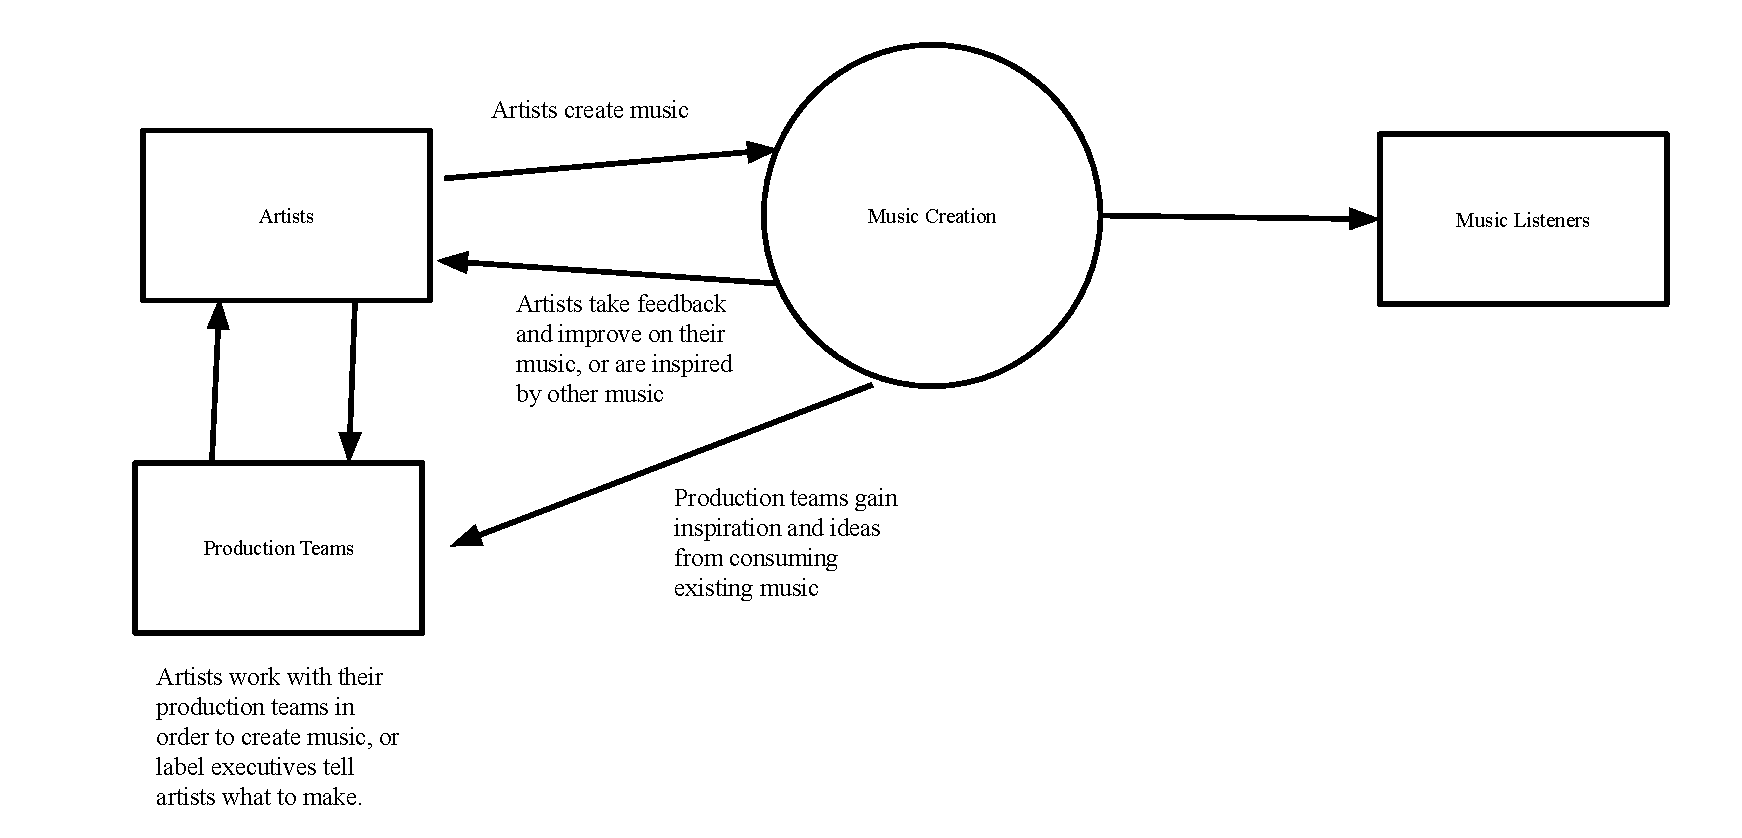
\includegraphics[width=\textwidth]{6_1_c.pdf}

\end{itemize}

\subsection{The Context of the Work}
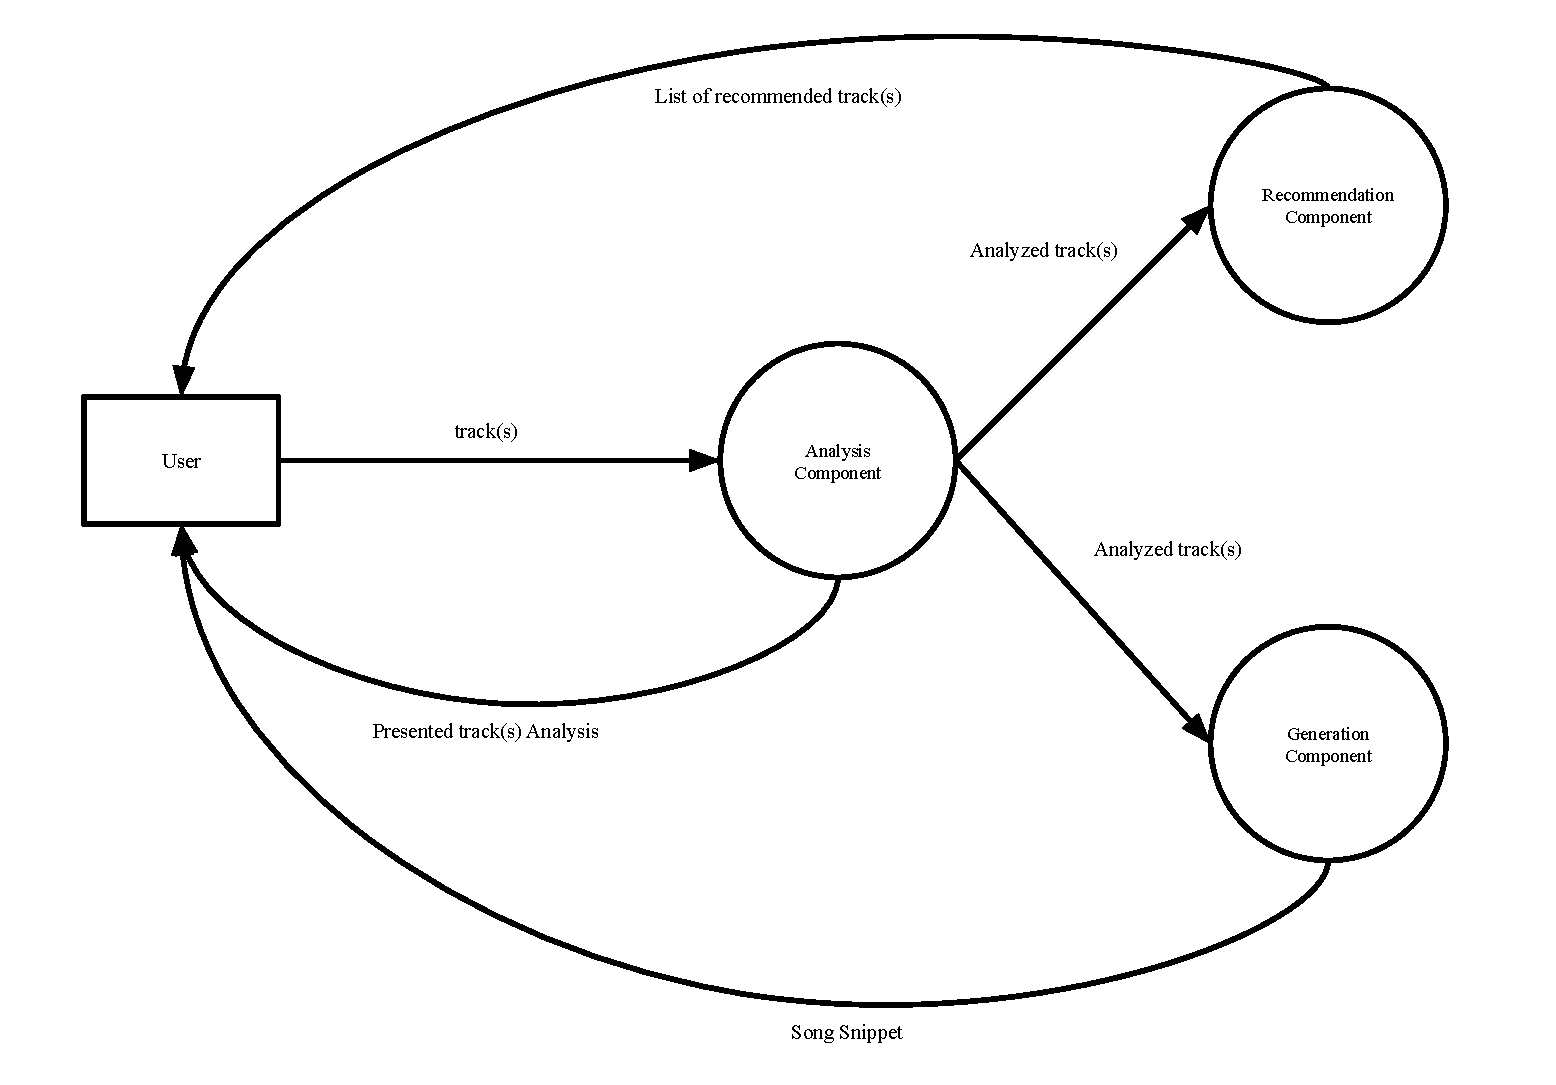
\includegraphics[width=\textwidth]{6_2_context_diagram.pdf}

\subsection{Work Partitioning}
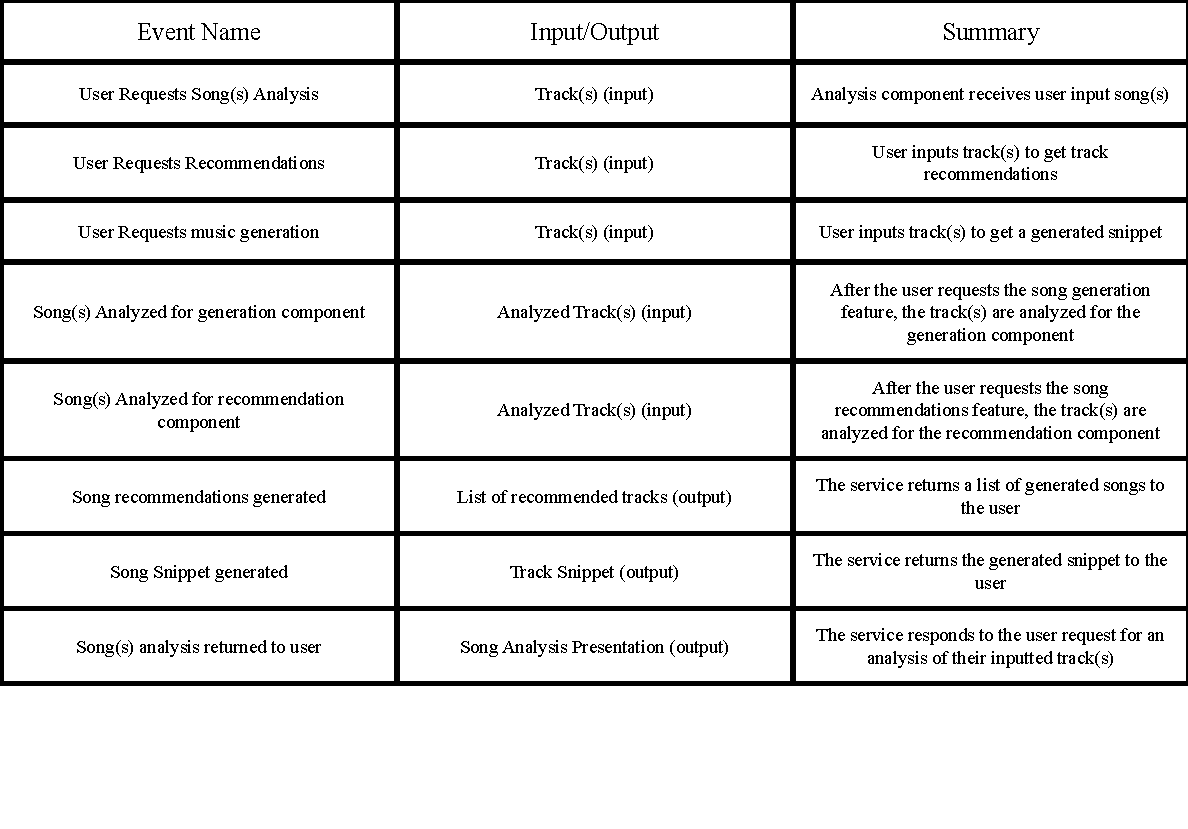
\includegraphics[width=\textwidth]{6_3_work_partitioning_table.pdf}

\subsection{Specifying a Business Use Case (BUC)}
\begin{itemize}
  \item \textbf{User Requests Track Recommendations}
    \\Primary Actor: App User
    \\Trigger: User intiates a request with the service to generate some new songs to listen to. 
    \\Preconditions: 
    \begin{itemize}
    \item User has valid references to tracks for the service to accept
    \item ML generation components are currently active
    \end{itemize}

    Main Success Scenario: 
    \begin{itemize}
    \item user submits request for track recommendation
    \item user inputs track(s) to the service
    \item the service's analyzation component analyzes the tracks
    \item analyzation component passes on tracks \& analysis to recommendation component
    \item recommendation component generates tracks
    \item user receives new tracks to listen to
    \end{itemize}
  
  \item \textbf{User Requests Track Analysis}
    \\Primary Actor: App User
    \\Trigger: User intiates a request with the service to generate some new songs to listen to. 
    \\Preconditions: 
    \begin{itemize}
    \item User has valid references to tracks for the service to accept
    \item ML generation components are currently active
    \end{itemize}

    Main Success Scenario: 
    \begin{itemize}
    \item user submits request for track recommendation
    \item user inputs track(s) to the service
    \item the service's analyzation component analyzes the tracks
    \item analyzation component generates presentations and visualizations based on the inputted track(s)
    \item the service returns generated presentations and visualizations to the user
    \end{itemize}
  
  \item \textbf{User Requests Snippet Generation}
    \\Primary Actor: App User
    \\Trigger: User intiates a request with the service to generate some new songs to listen to. 
    \\Preconditions: 
    \begin{itemize}
    \item User has valid references to tracks for the service to accept
    \item ML generation components are currently active
    \end{itemize}

    Main Success Scenario: 
    \begin{itemize}
    \item user submits request for snippet generation
    \item user inputs track(s) to the service
    \item the service's analyzation component analyzes the tracks
    \item analyzation component passes on tracks \& analysis to generation component
    \item generation component generates tracks
    \item user receives a snippet to listen to
    \end{itemize}
\end{itemize}



\section{Business Data Model and Data Dictionary}
\subsection{Business Data Model}
\lips
\subsection{Data Dictionary}
\lips

\section{The Scope of the Product}
\subsection{Product Boundary}
\lips
\subsection{Product Use Case Table}
\lips
\subsection{Individual Product Use Cases (PUC's)}
\lips

\section{Functional Requirements}
\subsection{Functional Requirements}
\lips

\section{Look and Feel Requirements}
\subsection{Appearance Requirements}
\lips
\subsection{Style Requirements}
\lips

\section{Usability and Humanity Requirements}
\subsection{Ease of Use Requirements}
\lips
\subsection{Personalization and Internationalization Requirements}
\lips
\subsection{Learning Requirements}
\lips
\subsection{Understandability and Politeness Requirements}
\lips
\subsection{Accessibility Requirements}
\lips

\section{Performance Requirements}
\subsection{Speed and Latency Requirements}
\lips
\subsection{Safety-Critical Requirements}
\lips
\subsection{Precision or Accuracy Requirements}
\lips
\subsection{Robustness or Fault-Tolerance Requirements}
\lips
\subsection{Capacity Requirements}
\lips
\subsection{Scalability or Extensibility Requirements}
\lips
\subsection{Longevity Requirements}
\lips

\section{Operational and Environmental Requirements}
\subsection{Expected Physical Environment}
\lips
\subsection{Wider Environment Requirements}
\lips
\subsection{Requirements for Interfacing with Adjacent Systems}
\lips
\subsection{Productization Requirements}
\lips
\subsection{Release Requirements}
\lips

\section{Maintainability and Support Requirements}
\subsection{Maintenance Requirements}
\lips
\subsection{Supportability Requirements}
\lips
\subsection{Adaptability Requirements}
\lips

\section{Security Requirements}
\subsection{Access Requirements}
\lips
\subsection{Integrity Requirements}
\lips
\subsection{Privacy Requirements}
\lips
\subsection{Audit Requirements}
\lips
\subsection{Immunity Requirements}
\lips

\section{Cultural Requirements}
\subsection{Cultural Requirements}
\lips

\section{Compliance Requirements}
\subsection{Legal Requirements}
\lips
\subsection{Standards Compliance Requirements}
\lips

\section{Open Issues}
\lips

\section{Off-the-Shelf Solutions}
\subsection{Ready-Made Products}
\lips
\subsection{Reusable Components}
\lips
\subsection{Products That Can Be Copied}
\lips

\section{New Problems}
\subsection{Effects on the Current Environment}
\lips
\subsection{Effects on the Installed Systems}
\lips
\subsection{Potential User Problems}
\lips
\subsection{Limitations in the Anticipated Implementation Environment That May
Inhibit the New Product}
\lips
\subsection{Follow-Up Problems}
\lips

\section{Tasks}
\subsection{Project Planning}
\lips
\subsection{Planning of the Development Phases}
\lips

\section{Migration to the New Product}
\subsection{Requirements for Migration to the New Product}
There are no migration requirements as this project is not a replacement or upgrade of a previous project
\subsection{Data That Has to be Modified or Translated for the New System}
Similarly, there currently is no data that needs to be modified

\section{Costs}
\lips
\section{User Documentation and Training}
\subsection{User Documentation Requirements}
\lips
\subsection{Training Requirements}
\lips

\section{Waiting Room}
\lips

\section{Ideas for Solution}
\lips

\newpage{}
\section*{Appendix --- Reflection}

The information in this section will be used to evaluate the team members on the
graduate attribute of Lifelong Learning.  Please answer the following questions:

\begin{enumerate}
  \item What knowledge and skills will the team collectively need to acquire to
  successfully complete this capstone project?  Examples of possible knowledge
  to acquire include domain specific knowledge from the domain of your
  application, or software engineering knowledge, mechatronics knowledge or
  computer science knowledge.  Skills may be related to technology, or writing,
  or presentation, or team management, etc.  You should look to identify at
  least one item for each team member.
  \item For each of the knowledge areas and skills identified in the previous
  question, what are at least two approaches to acquiring the knowledge or
  mastering the skill?  Of the identified approaches, which will each team
  member pursue, and why did they make this choice?
\end{enumerate}

\end{document}